\lecture{8}{28 Oct. 13:20}{}

\begin{definition}[2T]
    Let $V, W$ be vector spaces over a field $\mathbb{F}$. A linear transform from $V$ to $W$ is a function $T: V \to W$ such that preserves the operations on $V$ and $W$, i.e.
    \[
        \begin{cases}
            T(\mathbf{u} + \mathbf{v}) = T(\mathbf{u}) + T(\mathbf{v}), & \forall\ \mathbf{u}, \mathbf{v} \in V; \\
            T(c\mathbf{u}) = cT(\mathbf{u}), & \forall\ \mathbf{u} \in V, c \in \mathbb{F}.
        \end{cases}
    \]
\end{definition}

\begin{eg}
    \[
        T: \mathbb{R}^3 \to \mathbb{R}^3
    \]
    \[
        T: (x_1, x_2, x_3) \mapsto (x_2, x_3, x_1)
    \]
\end{eg}
T is a linear transform.

\begin{eg}
    \[
        A = \frac{d}{dt}: \mathbb{P}_n(\mathbb{R}) \to \mathbb{P}_{n-1}(\mathbb{R})
    \]
    \[
        p(t) \in \mathbb{P}_n(\mathbb{R}), \ p(t) = a_0 + a_1 t + a_2 t^2 + \cdots + a_n t^n
    \]
\end{eg}
See the attributes below:
\[
    AP = \frac{d}{dt} (a_0 + a_1 t + a_2 t^2 + \cdots + a_n t^n) = a_1 + 2a_2 t + \cdots + n a_n t^{n-1}
\]
The nullspace of $A$ is all constant polynomials.
\[
    \mathcal{C}(AP) = \mathbb{P}_{n-1}(\mathbb{R})
\]
the basis is $\{1, t, t^2, \ldots, t^{n-1}\}$ and $\rank(\mathcal{C}(A)) = n$.
\[
    \text{nullity}(A) + \rank(A) = 1 + n = \dim(\mathbb{P}_n(\mathbb{R})).
\]

\begin{eg}
    \[
        A = \int_0^t: \mathbb{P}_n(\mathbb{R}) \to \mathbb{P}_{n+1}(\mathbb{R})
    \]  
\end{eg}
See the attributes below:
\[
    AP = \int_0^t (a_0 + a_1 t + a_2 t^2 + \cdots + a_n t^n)\ dt = a_0 t + \frac{a_1 t^2}{2} + \frac{a_2 t^3}{3} + \cdots + \frac{a_n t^{n+1}}{n+1} + C
\]
The nullspace of $A$ is all constant polynomials.
\[
    \mathcal{N}(AP) = \{0\}
\]
The range of $A$
\[
    \mathcal{C}(AP) = \mathbb{P}_{n+1}(\mathbb{R}) - \{\text{constant}\} / \{0\}
\]
\begin{eg}
    \[
        T: \mathbb{R}^3 \to \mathbb{R}
    \]
    \[
        T: (x_1, x_2, x_3) \mapsto 2x_1 + 3x_2 - x_3, \ x_i \in \mathbb{R}
    \]
\end{eg}
$T$ is a linear transform.
\newpage

\begin{eg}
    \[
        T: \mathbb{R}^3 \to \mathbb{R}
    \]
    \[
        T: (x_1, x_2, x_3) \mapsto 2x_1^2 + 3x_2 - x_3, \ x_i \in \mathbb{R}
    \]
\end{eg}
$T$ is NOT a linear transform.
\[
    \because \ T(x+y) \neq T(x) + T(y)
\]

\begin{theorem}
    Let $T: V \to W$ be a linear transform, where $V, W$ are vector spaces over a field $\mathbb{F}$.
    \begin{enumerate}[label=(\roman*)]
        \item If $M$ is a subspace of $V$, then
        \[
            T(M) = \{x \in W \mid \exists\ \mathbf{m} \in M, \text{ such that } T(\mathbf{m}) = x\}
        \]
        is a subspace of $W$.
        \item If $N$ is a subspace of $W$, then
        \[
            T^{-1}(N) = \{\mathbf{v} \in V \mid T(\mathbf{v}) \in N\}
        \]
        is a subspace of $V$.
    \end{enumerate}
\end{theorem}
\begin{proof}
    Here is the proof:
    \begin{enumerate}[label=(\roman*)]
        \item Let $M \leq V$, $y_1, y_2 \in T(M) \subseteq W$, and $\alpha \in \mathbb{F}$.
        \[
            y_1, y_2 \in T(M) \implies \exists x_1, x_2 \in M \ \text{s.t.}\ T(x_1) = y_1,\ T(x_2) = y_2
        \]
        Then
        \[
            T(\alpha x_1 + x_2) = \alpha T(x_1) + T(x_2)
        \]
        since $T$ is a linear transformation. \\
        Also
        \[
            \alpha x_1 + x_2 \in M
        \]
        since $M$ is a subspace of $V$. \\
        Therefore
        \[
            \alpha y_1 + y_2 = \alpha T(x_1) + T(x_2) = T(\alpha x_1 + x_2) \in T(M)
        \]
        so $T(M)$ is a subspace of $W$.

        \item Let $x_1, x_2 \in T^{-1}(N)$ and $\alpha \in \mathbb{F}$.
        \[
            T(\alpha x_1 + x_2) = \alpha T(x_1) + T(x_2) \in N
        \]
        since $N \leq W$ and $T(x_1), T(x_2) \in N$. \\
        Therefore
        \[
            \alpha x_1 + x_2 \in T^{-1}(N)
        \]
        and $T^{-1}(N)$ is a subspace of $V$.
    \end{enumerate}
\end{proof}

\newpage

\begin{definition}
    $T: V \to W$ over a field $\mathbb{F}$ is a linear transform. Then $T^{-1}(\mathbf{O}_W)$ is called the \redbox{nullspace (kernel) of $T$}, where $\mathbf{O}_W$ is the zero vector in $W$. $T(V)$ is called the \redbox{range (image) of $T$}.
    \[
        \dim(T^{-1}(\mathbf{O}_W)) = \text{nullity}(T)
    \]
    \[
        \dim(T(V)) = \rank(T)
    \]
\end{definition}

\subsection{Matrix Representation of Linear Transformations}

\begin{exercise}
    What is the transformation taken $A: \mathbb{R}^2 \to \mathbb{R}^3$
    \[
        x_1 = \begin{pmatrix}
            1 \\ 0
        \end{pmatrix}_{\in \mathbb{R}^2} \ \to \ \begin{pmatrix}
            2 \\ 3 \\ 4
        \end{pmatrix}_{\in \mathbb{R}^3}, \quad
        x_2 = \begin{pmatrix}
            0 \\ 1
        \end{pmatrix}_{\in \mathbb{R}^2} \to \ \begin{pmatrix}
            4 \\ 6 \\ 8
        \end{pmatrix}_{\in \mathbb{R}^3}
    \]
\end{exercise}
\begin{answer}
    \[
        A = \begin{pmatrix}
            2 & 4 \\
            3 & 6 \\
            4 & 8
        \end{pmatrix}_{3 \times 2} = \left( T \right)_{\{e_1, e_2\}}^{\{e_1, e_2, e_3\}}
    \]
\end{answer}

\begin{eg}
    \[
        T: \mathbb{P}_3(\mathbb{R}) \to \mathbb{P}_2(\mathbb{R}), \ \text{ i.e. } T(f) = \frac{d}{dt} (f)
    \]
\end{eg}
The ordered basis of two vector spaces are
\[
    \begin{cases}
        \mathcal{B}_1 = \mathcal{B}(\mathbb{P}_3(\mathbb{R})): & \{1, t, t^2, t^3\} \\
        \mathcal{B}_2 = \mathcal{B}(\mathbb{P}_2(\mathbb{R})): & \{1, t, t^2\}
    \end{cases}
\]
Then we have
\[
    \begin{pmatrix}
        T
    \end{pmatrix}_{\blue{\mathcal{B}_2}}^{\blue{\mathcal{B}_1}} = \begin{matrix} 
        \red{1} \\ \red{t} \\ \red{t^2}
    \end{matrix}
    \begin{pmatrix}
        \overset{\red{1}}{0} & \overset{\red{t}}{1} & \overset{\red{t^2}}{0} & \overset{\red{t^3}}{0} \\
        0 & 0 & 2 & 0 \\
        0 & 0 & 0 & 3
    \end{pmatrix}_{3 \times 4} \quad \quad \text{e.g. }
    \begin{pmatrix}
        T
    \end{pmatrix} \begin{pmatrix}
        1 \\ 1 \\ 1 \\ 1
    \end{pmatrix} = \begin{pmatrix}
        1 \\ 2 \\ 3
    \end{pmatrix}_{3 \times 1}
\]

\begin{eg}
    \[
        T: \mathbb{P}_3(\mathbb{R}) \to \mathbb{P}_3(\mathbb{R}), \ \text{ i.e. } T(f) = \frac{d}{dt} (f)
    \]
\end{eg}
We have to handle the $t^3$ term, which means
\[
    \begin{pmatrix}
        T
    \end{pmatrix}_{\blue{\mathcal{B}_1}}^{\blue{\mathcal{B}_1}} = \begin{pmatrix}
        T
    \end{pmatrix}_{\blue{\mathcal{B}_1}} = \begin{matrix} 
        \red{1} \\ \red{t} \\ \red{t^2} \\ \red{t^3}
    \end{matrix}
    \begin{pmatrix}
        \overset{\red{1}}{0} & \overset{\red{t}}{1} & \overset{\red{t^2}}{0} & \overset{\red{t^3}}{0} \\
        0 & 0 & 2 & 0 \\
        0 & 0 & 0 & 3 \\
        0 & 0 & 0 & 0
    \end{pmatrix}_{4 \times 4}, \quad \quad \text{ this is called a } \blue{\langle \text{differentiation matrix} \rangle}
\]

\newpage

\begin{eg}
    \[
        \int_0^t: \mathbb{P}_3(\mathbb{R}) \to \mathbb{P}_4(\mathbb{R})
    \]
\end{eg}
The ordered basis of two vector spaces are
\[
    \begin{cases}
        \mathcal{B}_1 = \mathcal{B}(\mathbb{P}_3(\mathbb{R})): & \{1, t, t^2, t^3\}, \quad \dim(\mathbb{P}_3(\mathbb{R})) = 4 \\
        \mathcal{B}_2 = \mathcal{B}(\mathbb{P}_4(\mathbb{R})): & \{1, t, t^2, t^3, t^4\}, \quad \dim(\mathbb{P}_4(\mathbb{R})) = 5
    \end{cases}
\]
hence we have
\[
    \begin{pmatrix}
        T
    \end{pmatrix}_{\blue{\mathcal{B}_2}}^{\blue{\mathcal{B}_1}} = \begin{matrix} 
        \red{1} \\ \red{t} \\ \red{t^2} \\ \red{t^3} \\ \red{t^4}
    \end{matrix}
    \begin{pmatrix}
        \overset{\red{1}}{0} & \overset{\red{t}}{1} & \overset{\red{t^2}}{0} & \overset{\red{t^3}}{0} \\
        0 & 0 & \frac{1}{2} & 0 \\
        0 & 0 & 0 & \frac{1}{3} \\
        0 & 0 & 0 & 0 \\
        0 & 0 & 0 & \frac{1}{4}
    \end{pmatrix}_{5 \times 4} \quad \quad \text{which is called an } \blue{\langle \text{integration matrix} \rangle}
\]
and we also have
\[
    \mathcal{C}(T) = \text{span}\{t, t^2, t^3, t^4\}, \quad \rank(T) = 4
\]
\[
    \mathcal{N}(T) = \{0\}, \quad \text{nullity}(T) = 0
\]

\begin{eg}
    \[
        \mathbb{P}_2(\mathbb{R}) \xrightarrow{\int_t} \mathbb{P}_3(\mathbb{R}) \xrightarrow{\frac{d}{dt}} \mathbb{P}_2(\mathbb{R})
    \]
\end{eg}

\[
\begin{pmatrix}
    \frac{d}{dt} \ \int_0^t
\end{pmatrix} = \begin{pmatrix}
    \frac{d}{dt}
\end{pmatrix}_{3 \times 4} \begin{pmatrix}
    \int_0^t
\end{pmatrix}_{4 \times 3} = \begin{pmatrix}
    I 
\end{pmatrix}_{3 \times 3} \quad \text{Diff is the left inverse of Int}
\]

\subsection{Rotation $Q$, Projection $P$, Reflection $R$}
We introduce three important linear transformations in $\mathbb{R}^2$:
\[
    Q = \begin{pmatrix}
        \cos \theta & -\sin \theta \\
        \sin \theta & \cos \theta
    \end{pmatrix}, \quad P = \begin{pmatrix}
        1 & 0 \\
        0 & 0
    \end{pmatrix}, \quad R = \begin{pmatrix}
        1 & 0 \\
        0 & -1
    \end{pmatrix}
\]

\begin{enumerate}[label=$\arabic*^\circ$]
    \item Rotation: $Q$ rotates vectors by an angle $\theta$.
    \[
        \begin{pmatrix}
            Q
        \end{pmatrix} = \begin{pmatrix}
            \cos \theta & -\sin \theta \\
            \sin \theta & \cos \theta
        \end{pmatrix}_{2 \times 2}
    \]
    
    \begin{figure}[H]
        \centering
        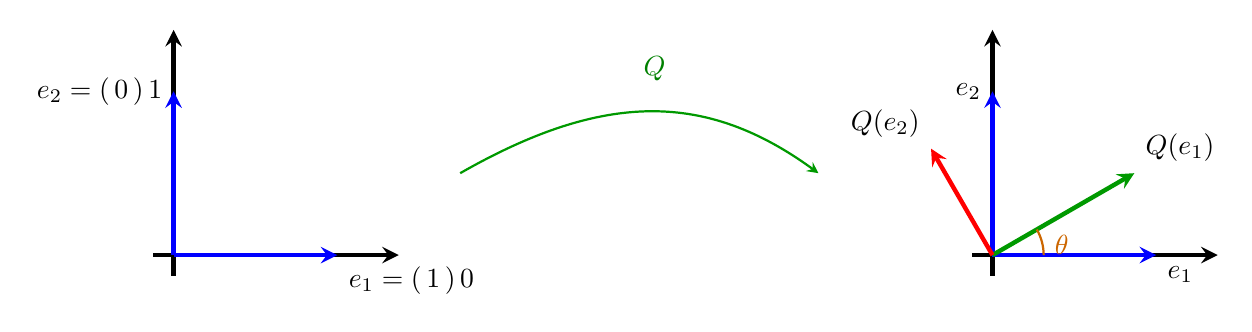
\begin{tikzpicture}[>=stealth, thick, scale=1.3]
    
        % === 左邊座標系 ===
        % 黑色主軸
        \draw[->, ultra thick] (0,-0.2) -- (0,2.2);
        \draw[->, ultra thick] (-0.2,0) -- (2.2,0);
    
        % 原始 e1, e2
        \draw[->, ultra thick, blue] (0,0) -- (1.6,0) node[below right, black] {$e_1 = \begin{pmatrix}1\\0\end{pmatrix}$};
        \draw[->, ultra thick, blue] (0,0) -- (0,1.6) node[left, black] {$e_2 = \begin{pmatrix}0\\1\end{pmatrix}$};
    
        % === 中間箭頭 Q ===
        \draw[->, thick, green!60!black] (2.8,0.8) .. controls (4.2,1.6) and (5.2,1.6) .. (6.3,0.8);
        \node[green!50!black, above] at (4.7,1.6) {$Q$};
    
        % === 右邊座標系 ===
        \begin{scope}[xshift=8cm, yshift=0cm]
        % 黑色主軸
        \draw[->, ultra thick] (0,-0.2) -- (0,2.2);
        \draw[->, ultra thick] (-0.2,0) -- (2.2,0);
    
        % 原始 e1, e2
        \draw[->, ultra thick, blue] (0,0) -- (1.6,0) node[below right, black] {$e_1$};
        \draw[->, ultra thick, blue] (0,0) -- (0,1.6) node[left, black] {$e_2$};
    
        % 旋轉角度
        \def\ang{30} % 旋轉角度
    
        % Q(e1) and Q(e2)
        \draw[->, ultra thick, green!60!black] (0,0) -- ({1.6*cos(\ang)},{1.6*sin(\ang)})
            node[above right, black] {$Q(e_1)$};
        \draw[->, ultra thick, red] (0,0) -- ({-1.2*sin(\ang)},{1.2*cos(\ang)})
            node[above left, black] {$Q(e_2)$};
    
        % theta 標記
        \draw[orange!80!black, thick] (0.5,0) arc[start angle=0, end angle=\ang, radius=0.5];
        \node[orange!80!black] at ({0.7*cos(\ang/2)}, {0.4*sin(\ang/2)}) {$\theta$};
        \end{scope}
    
        \end{tikzpicture}
        \caption{Rotation in $\mathbb{R}^2$}
    \end{figure}

    \newpage

    \[
        Q \begin{pmatrix}
            1 \\ 0
        \end{pmatrix} = \begin{pmatrix}
            \cos \theta \\ \sin \theta
        \end{pmatrix}, \quad Q \begin{pmatrix}
            0 \\ 1
        \end{pmatrix} = \begin{pmatrix}
            -\sin \theta \\ \cos \theta
        \end{pmatrix}
    \]

    \begin{itemize}
        \item $Q_{-\theta} \cdot Q_{\theta} = \mathbf{1}_{\mathbb{R}^2}$
        \item $Q_{\theta} \cdot Q_{\theta} = Q_{2\theta}$
        \item $Q_{\theta} \cdot Q_{\phi} = Q_{\theta + \phi}$
    \end{itemize}

    \item Projection: $P$ projects vectors onto the $\theta$-line.
    
    \begin{figure}[H]
        \centering
        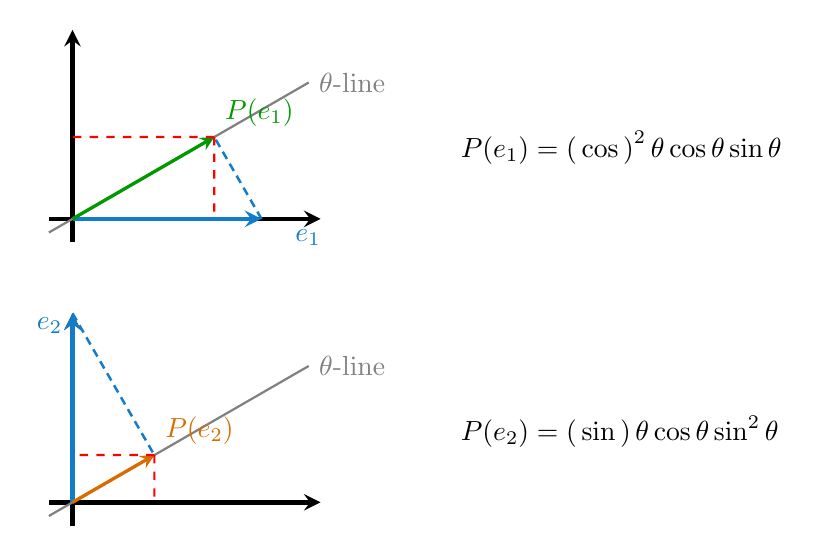
\begin{tikzpicture}[>=stealth, thick, scale=1.5]
        % -------- 共用參數 --------
        \def\ang{30}
        \def\L{1.6}
        \colorlet{axis}{black}
        \colorlet{eline}{cyan!60!blue}     % e1,e2顏色更亮
        \colorlet{tline}{gray}
        \colorlet{projone}{green!60!black}
        \colorlet{projtwo}{orange!85!black}
        
        % ======== 上圖: P(e1) ========
        \draw[->, ultra thick, axis] (-0.2,0) -- (2.1,0);
        \draw[->, ultra thick, axis] (0,-0.2) -- (0,1.6);
        
        % θ-line
        \draw[thick, tline] (-0.2,{-0.2*tan(\ang)}) -- (2, {2*tan(\ang)}) node[right, tline] {$\theta$-line};
        
        % e1 vector (更明顯)
        \draw[->, ultra thick, eline] (0,0) -- (\L,0);
        \node[eline, below right, font=\bfseries] at (1.8,0) {$e_1$};
        
        % e1 projection
        \coordinate (P1) at ({\L*cos(\ang)*cos(\ang)},{\L*cos(\ang)*sin(\ang)});
        \draw[->, very thick, projone] (0,0) -- (P1) node[above right] {$P(e_1)$};
        
        % e1 → θ-line 虛線
        \draw[eline, densely dashed, line width=0.9pt] (\L,0) -- (P1);
        
        % 輔助紅色虛線(垂足)
        \draw[red, dashed] (P1) -- ({\L*cos(\ang)*cos(\ang)},0);
        \draw[red, dashed] (P1) -- (0,{\L*cos(\ang)*sin(\ang)});
        
        % 結果矩陣
        \node[right] at (3.2,0.6)
        {$P(e_1)=
        \begin{pmatrix}
        \cos^2\theta\\[2pt]
        \cos\theta\sin\theta
        \end{pmatrix}$};
        
        % ======== 下圖: P(e2) ========
        \begin{scope}[yshift=-2.4cm]
        \draw[->, ultra thick, axis] (-0.2,0) -- (2.1,0);
        \draw[->, ultra thick, axis] (0,-0.2) -- (0,1.6);
        
        % θ-line
        \draw[thick, tline] (-0.2,{-0.2*tan(\ang)}) -- (2, {2*tan(\ang)}) node[right, tline] {$\theta$-line};
        
        % e2 vector (更明顯)
        \draw[->, ultra thick, eline] (0,0) -- (0,\L);
        \node[eline, left, font=\bfseries] at (0,1.5) {$e_2$};
        
        % e2 projection
        \coordinate (P2) at ({\L*sin(\ang)*cos(\ang)},{\L*sin(\ang)*sin(\ang)});
        \draw[->, very thick, projtwo] (0,0) -- (P2) node[above right] {$P(e_2)$};
        
        % e2 → θ-line 虛線
        \draw[eline, densely dashed, line width=0.9pt] (0,\L) -- (P2);
        
        % 輔助紅色虛線
        \draw[red, dashed] (P2) -- ({\L*sin(\ang)*cos(\ang)},0);
        \draw[red, dashed] (P2) -- (0,{\L*sin(\ang)*sin(\ang)});
        
        % 結果矩陣
        \node[right] at (3.2,0.6)
        {$P(e_2)=
        \begin{pmatrix}
        \sin\theta\cos\theta\\[2pt]
        \sin^2\theta
        \end{pmatrix}$};
        \end{scope}
        
        \end{tikzpicture}
        \caption{Projection onto a line at angle $\theta$}
    \end{figure}

    \[
        P = \begin{pmatrix}
            \cos^2 \theta & \sin \theta \cos \theta \\
            \sin \theta \cos \theta & \sin^2 \theta
        \end{pmatrix}
    \]

    Here are some properties of projection:
    \begin{itemize}
        \item $P^2 = P$
        \item Symmetric: $P^T = P$
        \item $P^{-1}$ does not exist.
    \end{itemize}

    \begin{enumerate}[label=$\arabic*^\circ$]
        \item \begin{align*}
        P \left( \alpha \begin{pmatrix}
            \cos \theta \\
            \sin \theta
        \end{pmatrix}  \right) &= \alpha P \begin{pmatrix}
            \cos \theta \\
            \sin \theta
        \end{pmatrix} \\ &= \alpha \begin{pmatrix}
            \cos^2 \theta & \sin \theta \cos \theta \\
            \sin \theta \cos \theta & \sin^2 \theta
        \end{pmatrix} \begin{pmatrix}
            \cos \theta \\
            \sin \theta
        \end{pmatrix} = \alpha \begin{pmatrix}
            \cos^3 \theta + \cos \theta \sin^2 \theta \\
            \sin \theta \cos^2 \theta + \sin^3 \theta
        \end{pmatrix} = \alpha \begin{pmatrix}
            \cos \theta \\
            \sin \theta
        \end{pmatrix}
        \end{align*}

        \item \begin{align*}
        P \left( \alpha \begin{pmatrix}
            -\sin \theta \\
            \cos \theta
        \end{pmatrix}  \right) &= \alpha P \begin{pmatrix}
            -\sin \theta \\
            \cos \theta
        \end{pmatrix} \\ &= \alpha \begin{pmatrix}
            \cos^2 \theta & \sin \theta \cos \theta \\
            \sin \theta \cos \theta & \sin^2 \theta
        \end{pmatrix} \begin{pmatrix}   
            -\sin \theta \\
            \cos \theta
        \end{pmatrix} = \alpha \begin{pmatrix}
            -\sin \theta \cos^2 \theta + \cos \theta \sin \theta \\
            -\sin^2 \theta \cos \theta + \sin^3 \theta
        \end{pmatrix} = \alpha \begin{pmatrix}
            0 \\
            0
        \end{pmatrix}
        \end{align*}
        Thus,
        \[
            \boxed{\alpha \begin{pmatrix}
                -\sin \theta \\
                \cos \theta
            \end{pmatrix} \quad \text{is in the nullspace of } P.}
        \]
    \end{enumerate}

    \newpage

    \item Reflection: $R$ reflects vectors across the $\theta$-line.
    
    \begin{figure}[H]
        \centering

        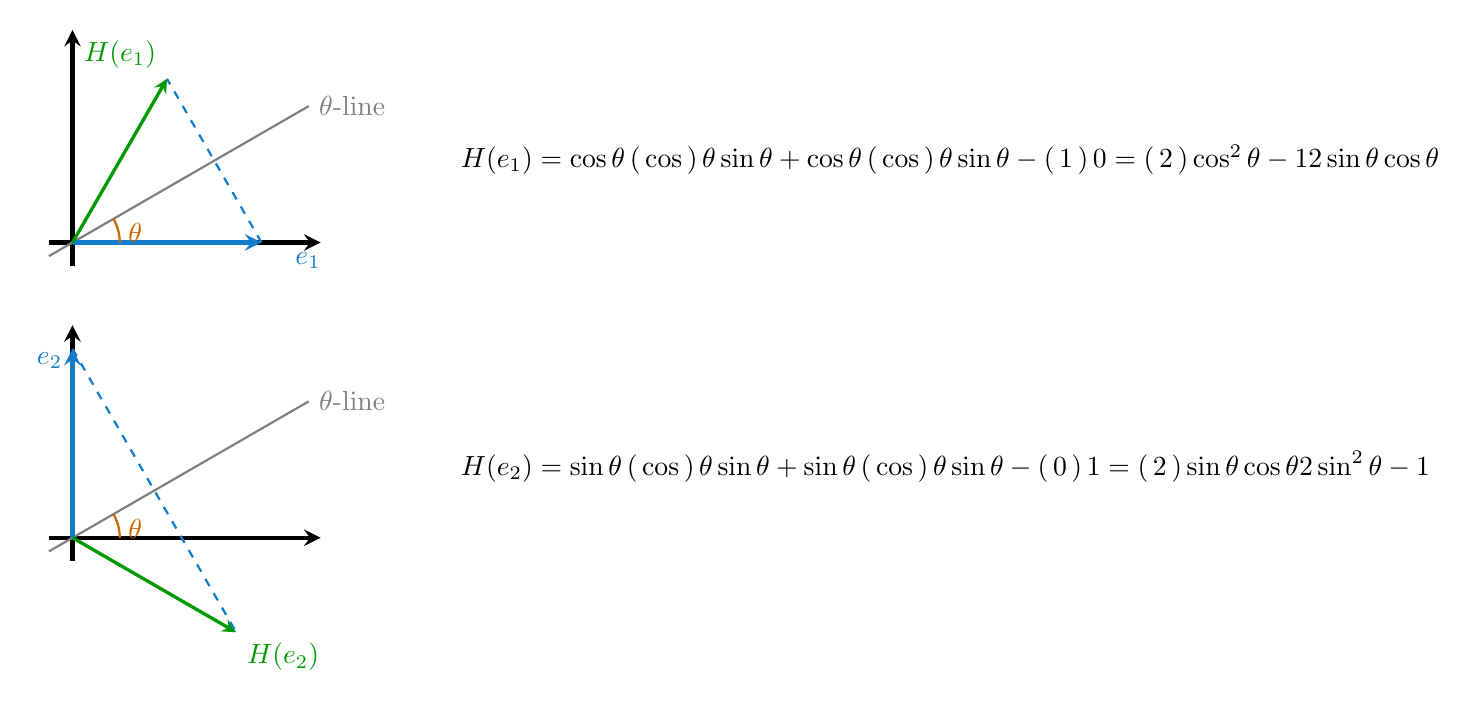
\begin{tikzpicture}[>=stealth, thick, scale=1.5]
        % ----------- 共用參數 -----------
        \def\ang{30}       % θ
        \def\L{1.6}        % 基準長度
        \colorlet{axis}{black}
        \colorlet{eline}{cyan!60!blue}
        \colorlet{tline}{gray}
        \colorlet{refone}{green!60!black}
        \colorlet{reftwo}{green!60!black}
        
        % =====================================
        %            上圖:H(e1)
        % =====================================
        \draw[->, ultra thick, axis] (-0.2,0) -- (2.1,0);
        \draw[->, ultra thick, axis] (0,-0.2) -- (0,1.8);
        
        % θ-line
        \draw[thick, tline] (-0.2,{-0.2*tan(\ang)}) -- (2, {2*tan(\ang)}) node[right, tline] {$\theta$-line};
        
        % e1 向量
        \draw[->, ultra thick, eline] (0,0) -- (\L,0);
        \node[eline, below right, font=\bfseries] at (1.8,0) {$e_1$};
        
        % 反射後向量 H(e1)
        \coordinate (R1) at ({\L*cos(2*\ang)},{\L*sin(2*\ang)});
        \draw[->, very thick, refone] (0,0) -- (R1) node[above left] {$H(e_1)$};
        
        % 藍色虛線:反射前後對稱
        \draw[eline, dashed] (\L,0) -- (R1);
        
        % 角度 θ 標示
        \draw[orange!80!black, thick] (0.4,0) arc[start angle=0, end angle=\ang, radius=0.4];
        \node[orange!80!black] at ({0.55*cos(\ang/2)}, {0.3*sin(\ang/2)}) {$\theta$};
        
        % 結果矩陣
        \node[right] at (3.2,0.7)
        {$H(e_1)= \cos \theta
        \begin{pmatrix}
            \cos\theta \\
            \sin\theta
        \end{pmatrix} + \cos \theta
        \begin{pmatrix}
            \cos\theta \\
            \sin\theta
        \end{pmatrix} - \begin{pmatrix}
            1 \\
            0
        \end{pmatrix} =
        \begin{pmatrix}
        2\cos^2\theta-1\\[3pt]
        2\sin\theta\cos\theta
        \end{pmatrix}$};
        
        % =====================================
        %            下圖:H(e2)
        % =====================================
        \begin{scope}[yshift=-2.5cm]
        \draw[->, ultra thick, axis] (-0.2,0) -- (2.1,0);
        \draw[->, ultra thick, axis] (0,-0.2) -- (0,1.8);
        
        % θ-line
        \draw[thick, tline] (-0.2,{-0.2*tan(\ang)}) -- (2, {2*tan(\ang)}) node[right, tline] {$\theta$-line};
        
        % e2 向量
        \draw[->, ultra thick, eline] (0,0) -- (0,\L);
        \node[eline, left, font=\bfseries] at (0,1.5) {$e_2$};
        
        % 反射後 H(e2)
        \coordinate (R2) at ({\L*sin(2*\ang)},{-\L*cos(2*\ang)});
        \draw[->, very thick, reftwo] (0,0) -- (R2) node[below right] {$H(e_2)$};
        
        % 虛線連接對稱
        \draw[eline, dashed] (0,\L) -- (R2);
        
        % θ 標示
        \draw[orange!80!black, thick] (0.4,0) arc[start angle=0, end angle=\ang, radius=0.4];
        \node[orange!80!black] at ({0.55*cos(\ang/2)}, {0.3*sin(\ang/2)}) {$\theta$};
        
        % 結果矩陣
        \node[right] at (3.2,0.6)
        {$H(e_2)=\sin \theta
        \begin{pmatrix}
            \cos\theta \\
            \sin\theta
        \end{pmatrix} + \sin \theta
        \begin{pmatrix}
            \cos\theta \\
            \sin\theta
        \end{pmatrix} - 
        \begin{pmatrix}
            0 \\
            1
        \end{pmatrix} = 
        \begin{pmatrix}
        2\sin\theta\cos\theta \\
        2\sin^2\theta-1
        \end{pmatrix}$};
        \end{scope}
        
        \end{tikzpicture}
        \caption{Reflection across a line at angle $\theta$}
    \end{figure}

    \[
        H = \begin{pmatrix}
            2\cos^2 \theta - 1 & 2\sin \theta \cos \theta \\
            2\sin \theta \cos \theta & 2\sin^2 \theta - 1
        \end{pmatrix}
    \]

    Here are some properties of reflection:
    \begin{itemize}
        \item $H^2 = I$
        \item $H^{-1} = H$
        \item $H = 2P - I\ (Hx + x = 2Px)$
    \end{itemize}

\end{enumerate}

\begin{note}
    If first basis vector is on the $\theta$-line, and the second basis vector is perpendicular to the $\theta$-line, then
    \[
        P^* = \begin{pmatrix}
            1 & 0 \\
            0 & 0
        \end{pmatrix}, \quad H^* = \begin{pmatrix}
            1 & 0 \\
            0 & -1
        \end{pmatrix} = 2P^* - I, \quad Q^* = \begin{pmatrix}
            \cos \theta & -\sin \theta \\
            \sin \theta & \cos \theta   
        \end{pmatrix}
    \]
\end{note}

\newpage

\chapter{Orthogonality}
\section{Perpendicular Vectors and Orthogonal Subspaces}

There are three important concepts in this section:
\begin{enumerate}[label=(\roman*)]
    \item The length of vector
    \item The test for perpendicularity
    \item How to create perpendicular vectors form linearly independent vectors
\end{enumerate}

Now we start to discuss:
\begin{enumerate}[label=(\roman*)]
    \item \textbf{The length of vector}:\\
    The length (or norm) of a vector, in $\mathbb{R}^n$, that satisfies the Pythagorean theorem is defined as:
    \begin{definition}
        Let $\mathbf{x} \in \mathbb{R}^n$ be
        \[
            \mathbf{x} = (x_1, x_2, \ldots, x_n) = x_1 e_1 + x_2 e_2 + \cdots + x_n e_n \in \mathbb{R}^n 
        \]
        then
        \[
            \|\mathbf{x}\|^2 = \sum_{i=1}^n x_i^2 = \mathbf{x}^T \mathbf{x}
        \] 
    \end{definition}

    \item \textbf{The test for perpendicularity}:\\
    \begin{definition}
        Given $\mathbf{x}, \mathbf{y} \in \mathbb{R}^n$, then if $\mathbf{x} \perp \mathbf{y}$, then by Pythagorean theorem, we have
        \[
            \|\mathbf{x}\|^2 + \|\mathbf{y}\|^2 = \|\mathbf{x} - \mathbf{y}\|^2
        \]
        Then we can deduce that 
        \[
            x_1^2 + x_2^2 + \cdots + x_n^2 + y_1^2 + y_2^2 + \cdots + y_n^2 = (x_1 - y_1)^2 + (x_2 - y_2)^2 + \cdots + (x_n - y_n)^2
        \]
        then we have
        \[
            \mathbf{x}^T \mathbf{y} = 0
        \]
    \end{definition}
\end{enumerate}

\newpage

\begin{definition}[Inner Product]
    Let $V$ be a vector space over a field $\mathbb{F}\ (\mathbb{R}, \mathbb{C})$. An inner product on $V$ is a function that assigns to every ordered pair of vectors $\mathbf{x}$ and $\mathbf{y}$ in $V$, a scalar in $\mathbb{F}$, denoted as 
    \[
        \langle \mathbf{x}, \mathbf{y} \rangle
    \]
    \( \forall\ \mathbf{x}, \mathbf{y}, \mathbf{z} \in V, \ c \in \mathbb{F} \), we have
    \begin{enumerate}[label=(\alph*)]
        \item $\langle \mathbf{x} + \mathbf{y}, \mathbf{z} \rangle = \langle \mathbf{x}, \mathbf{z} \rangle + \langle \mathbf{y}, \mathbf{z} \rangle$
        \item $\langle c\ \mathbf{x}, \mathbf{y} \rangle = c\ \langle \mathbf{x}, \mathbf{y} \rangle$
        \item $\langle \mathbf{y}, \mathbf{x} \rangle = \overline{\langle \mathbf{x}, \mathbf{y} \rangle}$ (where $\overline{a + bi} = a - bi$ complex conjugate)
        \item $\langle \mathbf{x}, \mathbf{x} \rangle > 0$, if $\mathbf{x} \neq \mathbf{0}$
    \end{enumerate}
\end{definition}

\begin{note}[1]
    If $\mathbb{F} = \mathbb{R}$, (c) will reduce to $\langle \mathbf{y}, \mathbf{x} \rangle = \langle \mathbf{x}, \mathbf{y} \rangle$.
\end{note}

\begin{note}[2]
    Inner product is \blue{linear} in the first component.
\end{note}

\begin{definition}[Standard Inner Product]
    Let $V = \mathbb{R}^n / \mathbb{R}$, defined 
    \[
        \langle \mathbf{x}, \mathbf{y} \rangle = \mathbf{x}^T \mathbf{y} = \sum_{i=1}^{n} x_i y_i    
    \]
    This is called the \redbox{standard inner product} on $\mathbb{R}^n$.
\end{definition}

\begin{proposition}
    If $\mathbf{x}, \mathbf{y} \in \mathbb{R}^n$, then
    \begin{itemize}
        \item Let $\langle \mathbf{x}, \mathbf{y} \rangle = x^Ty$ be standard inner product.
        \item Let $\langle \mathbf{x}, \mathbf{y} \rangle = 0$ if and only if $\mathbf{x} \perp \mathbf{y}$.
    \end{itemize}
\end{proposition}

\begin{eg}
    If $\langle , \rangle$ is any inner product on $V$, and $r > 0$, we define \[
        \langle \mathbf{x},\mathbf{y} \rangle' = r \langle \mathbf{x}, \mathbf{y} \rangle
    \]
    \begin{enumerate}[label=$\arabic*^\circ$]
        \item $\langle \mathbf{x} + \mathbf{y}, \mathbf{z} \rangle' = r \langle \mathbf{x} + \mathbf{y}, \mathbf{z} \rangle = r \langle \mathbf{x}, \mathbf{z} \rangle + r \langle \mathbf{y}, \mathbf{z} \rangle = \langle \mathbf{x}, \mathbf{z} \rangle' + \langle \mathbf{y}, \mathbf{z} \rangle'$
        \item $\langle c\mathbf{x}, \mathbf{y} \rangle' = r \langle c\mathbf{x}, \mathbf{y} \rangle = c \cdot r \langle \mathbf{x}, \mathbf{y} \rangle = c \langle \mathbf{x}, \mathbf{y} \rangle'$
    \end{enumerate}
\end{eg}

\begin{eg}
    Let $V = \{ f \mid f: \text{real-valued continuous functions on } [0,1] \} = \mathcal{C}([0,1])$. For $f, g \in V$, define
    \[
        \langle f, g \rangle = \int_0^1 f(t) g(t) dt
    \]
\end{eg}

\begin{eg}
    Let $V = \mathbb{C}^n$, $\mathbb{C}^n$ is a vector space over $\mathbb{C}$. For $\mathbf{x}, \mathbf{y} \in V$, define
    \[
        \langle \mathbf{x}, \mathbf{y} \rangle = \mathbf{x}^T \overline{\mathbf{y}} = \sum_{i=1}^n x_i \overline{y_i}
    \]
    \[
        \langle \mathbf{y}, \mathbf{x} \rangle
        = \mathbf{y}^\mathsf{T} \overline{\mathbf{x}}
        = \overline{\,\mathbf{x}^\mathsf{T} \overline{\mathbf{y}}\,}
        = \overline{\langle \mathbf{x}, \mathbf{y} \rangle}.
    \]
\end{eg}

\newpage

\begin{eg}
    Let $V = \mathbb{C}$, $\mathbb{C}$ is a vector space over $\mathbb{C}$. If $\mathbf{x}, \mathbf{y} \in \mathbb{C}$, $x = a+bi$, $y = c+di$, define
    \[
        \langle \mathbf{x}, \mathbf{y} \rangle = (a + bi)(c - di)
    \]
    \begin{enumerate}[label=$\arabic*^\circ$]
        \item $\langle \mathbf{y}, \mathbf{x} \rangle = (c + di)(a - bi) = \overline{(a + bi)(c - di)} = \overline{\langle \mathbf{x}, \mathbf{y} \rangle}$
        \item $\langle \mathbf{x}, \mathbf{x} \rangle = (a + bi)(a - bi) = a^2 + b^2 > 0$ if $\mathbf{x} \neq 0$
    \end{enumerate}
\end{eg}